% Template for BiDS'19 papers; to be used with:
%          spconf.sty  - LaTeX style file, and
% --------------------------------------------------------------------------
\documentclass{article}
\usepackage{spconf,amsmath,epsfig}

\providecommand{\doi}[1]{doi: {\footnotesize \href{http://dx.doi.org/#1}{\path{#1}}}}

\usepackage[pdftex=true,breaklinks=true,hidelinks=true,colorlinks=true,citecolor=blue]{hyperref}

\usepackage[square,numbers]{natbib}
\renewcommand{\bibsection}{\section*{\normalsize\hspace*{\fill}REFERENCES\hspace*{\fill}}}


% Example definitions.
% --------------------
\def\x{{\mathbf x}}
\def\L{{\cal L}}

% Title.
% ------
\title{THE PANGEO BIG DATA ECOSYSTEM AND ITS USE AT CNES}
%
% Single address.
% ---------------
\name{Guillaume Eynard-Bontemps, Joseph Hamman, Ryan Abernathey, Matthew Rocklin, Aurélien Ponte}%\thanks{Thanks to XYZ agency for funding.}}
\address{CNES, NCAR, Columbia, Anaconda, Ifremer}
%
% For example:
% ------------
%\address{School\\
%	Department\\
%	Address}
%
% Two addresses (uncomment and modify for two-address case).
% ----------------------------------------------------------
%\twoauthors
%  {A. Author-one, B. Author-two\sthanks{Thanks to XYZ agency for funding.}}
%	{School A-B\\
%	Department A-B\\
%	Address A-B}
%  {C. Author-three, D. Author-four\sthanks{The fourth author performed the work
%	while at ...}}
%	{School C-D\\
%	Department C-D\\
%	Address C-D}
%
\begin{document}
%\ninept
%
\maketitle
%
\begin{abstract}
Pangeo\cite{b1} is a community driven effort for open-source big-data intially focused on the Earth System Sciences. It represents at the same time a collaboration of people and a platform composed of open source scientific python packages like Jupyter, Dask and Xarray. One of its goal is to improve scalability of these tools to handle petabyte-scale datasets on HPC or public cloud infrastructure.
In this paper, we will first describe Pangeo: its motivation, community, the underlying technology stack and associated deployments, different applications and the on going work. On a second part, we will present its use in CNES: HPC deployment, some simple and more complicated use cases, and what we are planning to do.
\end{abstract}
%
\begin{keywords}
Pangeo, Dask, Jupyter, HPC, Cloud, Big Data, Analysis
\end{keywords}
%
\section{Pangeo}
\label{sec:pangeo}

\subsection{Motivations, mission and goals}
\label{ssec:motivations}

There are several building crises facing the geoscience community:

\begin{itemize}
\item Big Data: datasets are growing too rapidly\ref{nasa_cloud_growth} and legacy software tools for scientific analysis can’t handle them. This is a major obstacle to scientific progress.
\item Technology Gap: a growing gap between the technological sophistication of industry solutions (high) and scientific software (low).
\item Reproducibility: a fragmentation of software tools and environments renders most geoscience research effectively unreproducible and prone to failure.
\end{itemize}

Pangeo aims to address these challenges through a unified, collaborative effort.

\begin{figure}
  \centering
  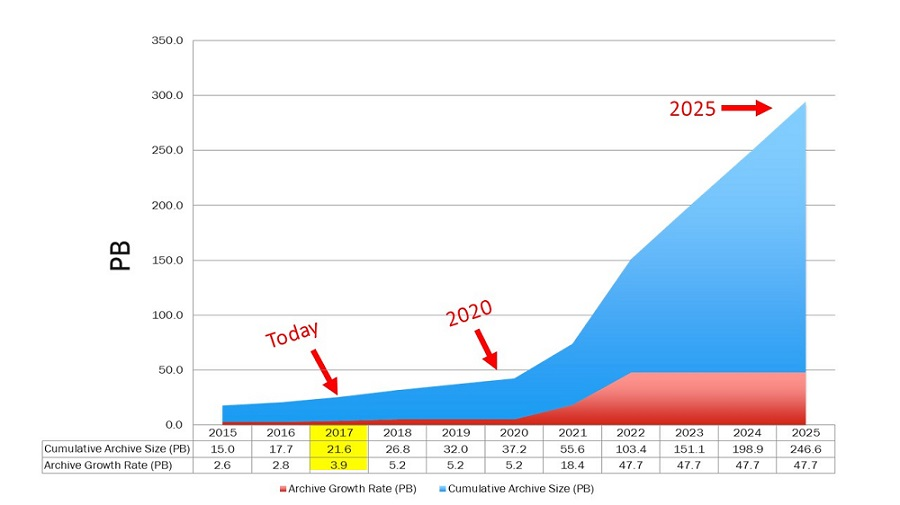
\includegraphics[width=\columnwidth]{EOSDIS_archive_growth_updated_resize.jpg}
  \caption{\label{nasa_cloud_growth} Projected NASA Earth Observing System Cloud storage\cite{b2}.}
\end{figure}

Our mission is to cultivate an ecosystem in which the next generation of open-source analysis tools for ocean, atmosphere and climate science can be developed, distributed, and sustained. These tools must be scalable in order to meet the current and future challenges of big data, and these solutions should leverage the existing expertise outside of the geoscience community.

To accomplish this mission, we have identified three specific goals.
\begin{itemize}
\item Foster collaboration around the open source scientific python ecosystem for ocean / atmosphere / land / climate science.
\item Support the development with domain-specific geoscience packages.
\item Improve scalability of these tools to handle petabyte-scale datasets on HPC and cloud platforms.
\end{itemize}

\subsection{Community}
\label{ssec:community}

One crutial attribute of Pangeo is to be community driven. The goal is of course to have the most wider and open collaboration as possible. All the effort are made in the open on github\cite{b3}, any one can join or get involved in the community. 

The community is already quite diverse, from academic research, going through government agency and to open source developers. A lot of different nationalities are represented too: from USA of course, but also UK, France or Australia to name a few.


\subsection{Technology stack}
\label{ssec:techstack}

Pangeo software ecosystem fits directly in the Scientific Python stack, involving well known modules such as Numpy, Pandas, or Sickit-learn\ref{scipy_stack}.

\begin{figure}
  \centering
  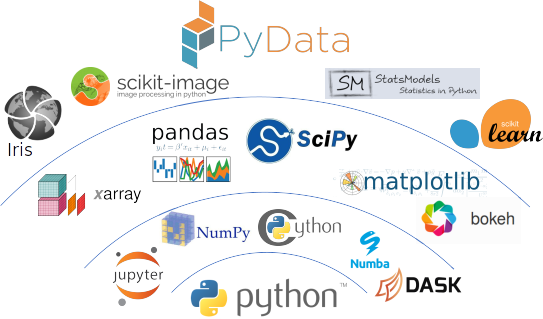
\includegraphics[width=\columnwidth]{pangeo_python_stack.png}
  \caption{\label{scipy_stack} Pangeo scientific Python ecosystem.}
\end{figure}

Three python software libraries are at the core of Pangeo:
\begin{itemize}
\item Jupyter notebooks and Jupyterhub allow interactive computing and analysis from a web application and user handling. They are quickly becoming the standard open-source format for interactive computing in Python.
\item Dask is a library for parallel computing that coordinates with Python’s existing scientific software ecosystem, including libraries cited above. In many cases, it offers users the ability to take existing workflows and quickly scale them to much larger applications. Dask-distributed is an extension of dask that facilitates parallel execution across many computers.
\item Xarray is the interface for working with big datasets: it offers a Pandas like API for dealing with labelled n-dimensionnasl array at scale.
\end{itemize}

The github community offers online documentation, scripts and other tooling to link them together in order to deploy a Pangeo platform\ref{pangeo_stack} and put the stack on HPC systems or in the public Cloud. The main elements allowing to build and use the platforms along the core libraries are:
\begin{itemize}
\item A set of scripts and documentation that allows automatically creating the necessary Cloud Infrastructure. Currently available for Google Cloud Engine, but a lot of work is being done for Amazon Web Services compatibility. There is also a lot of automation that the community is working on using Terraform software or CI/CD tooling.
\item Dask interfaces to automatically deploy distributed cluster allong various infrastructures: dask-kubernetes for Kubernetes cluster and so the public Cloud, dask-jobqueue\cite{b4} for HPC systems using scheduler such as Slurm, PBS Pro or LSF, and dask-yarn for Big Data infrastrucure.
\end{itemize}

\begin{figure}
  \centering
  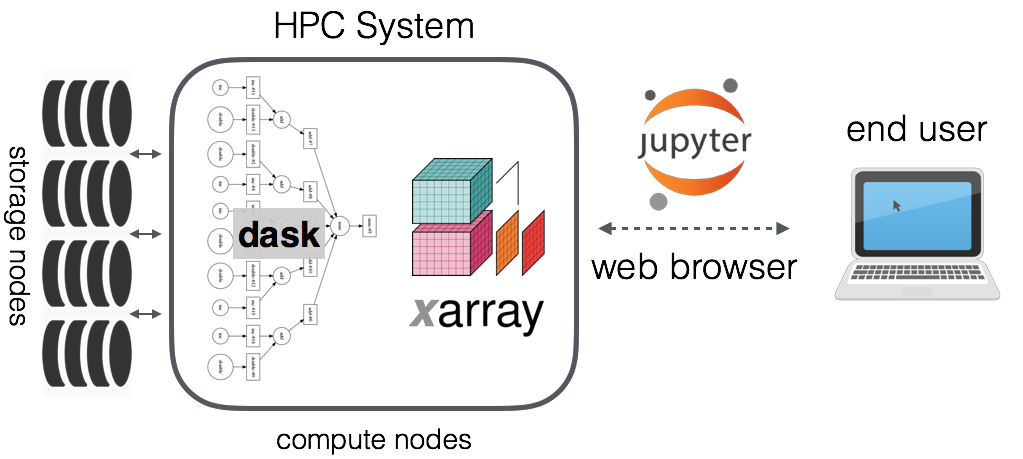
\includegraphics[width=\columnwidth]{pangeo_stack.png}
  \caption{\label{pangeo_stack} Pangeo platform main components.}
\end{figure}

\subsection{Applications}
\label{ssec:applications}

Pangeo first scientific domain is earth sciences: ocean, atmosphere, land or climate. There is already a lot of applications of the ecosystem in these domains. Some real science use cases can be found online\cite{b5} along their datasets and directly executed from a web browser. We can for example cite Sea Surface Altimetry Data Analysis that explore the increase of global mean sea level over 20 years of data, or also US Precipitation and Temperature Analysis that explore meteorological gridded ensemble precipitation and temperature estimates over the contiguous United States.

But other scientific domains are more and more interested by Pangeo possibilities:
\begin{itemize}
\item Satellite imagery analysis: there is a great blog post\cite{b6} explaining how to use Pangeo for processing and analysing in real time Landsat imagery. NASA has also decided to fund Pangeo initiative for applying the ecosystem on remote sensing datasets that are being put on AWS.
\item Astronomy: several scientists are already using the web platform to explore Gaia DR2 data on GCE.
\item Neuroscience: there is on going work to use Pangeo for analysis on human brain or electrophysiological datasets.
\end{itemize}

The principal point for allowing all this work is to dispose of a Cloud ready available dataset. This means that data must be accessible in a cloud or distributed storage friendly format, like Zarr for multi dimensionnal data, Cloud optimized Geotiff for satellite imagery, or Parquet for tabular data. See \cite{b7} for more details on this.

\subsection{On going work}
\label{ssec:ongowork}

The community is very active and working on improving Pangeo possibilities and accessibilities. This includes but does not limit to the following on going tasks:
\begin{itemize}
\item Active work for giving everyone the possibility to try to use Pangeo at scale. This is made possible by using Binder tools along with Pangeo ecosystem\cite{b8}. Binder allows anyone to launch a cloud environment and interactive notebook from a simple clic on a HTML link.
\item Community governance: Pangeo is still young, it needs further organization. Lot of work has begun on this in the last Pangeo developper meeting this summer.
\item As mentioned previously, Pangeo is an ecosystem that can be used by different scientific domains, each of thos having their own software stack. In order to cope with that, it has recently been decided to offer a specific cloud environment for all these different communitites.
\item In order to simplify the above point, a lot of work is currently being done on simplifying Cloud environment updates, by using mordern tooling for Continous Deployment.
\item As Pangeo is compatible not only with cloud but with different infrastructure, several Dask subcomponents share some logic for deploying clusters. A work to rationalize this logic and separated resources management from Dask scheduling is on going.
\end{itemize}

\section{CNES deployment and use cases}
\label{sec:cnes}

\subsection{Context and projects}
\label{ssec:context}

The Centre National d'Etudes Spatiales (CNES) is the government agency responsible for shaping and implementing France’s space policy in Europe. As such it covers a wide range of subjects: Ariane launcher, Sciences, Earth observation, telecommunication and defence.

On the ground segment processing side, we are involved on several Big Data projects, hosted or not in CNES Data Center:
\begin{itemize}
\item Gaia data processing center for some science unit,
\item Sentinel product Exploitation Platform, for sharing and online processing of copernicus products,
\item Surface Water and Ocean Topography (SWOT) mission, with French processing center hosted at CNES,
\item Euclid astronomy mission, for the architecture part.
\end{itemize}

We are also performing a lot of other processing involving remote sensing data, flight dynamics or other domain on our HPC cluster.

\subsection{Pangeo on HPC System}
\label{ssec:pangeohpc}

\begin{figure}
  \centering
  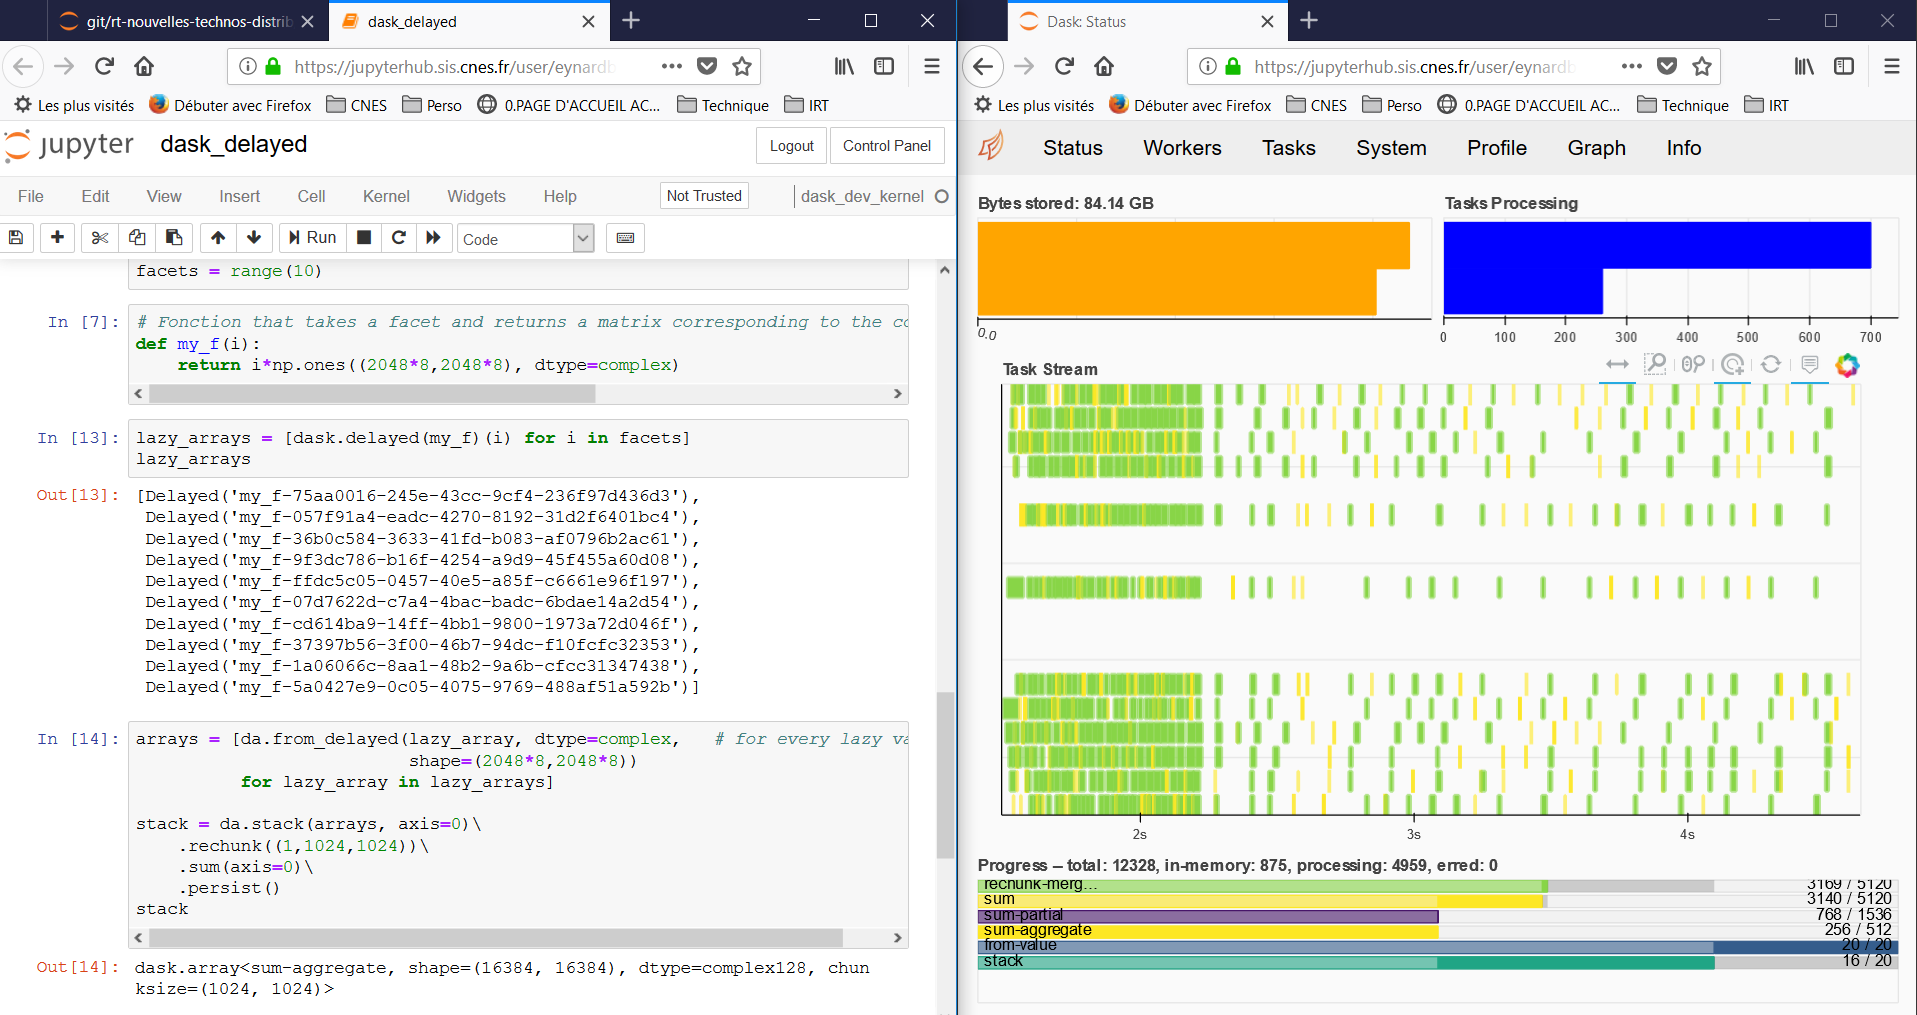
\includegraphics[width=\columnwidth]{dask_jobqueue.png}
  \caption{\label{dask_jobqueue} Notebook and Dask dashboard running with dask-jobqueue.}
\end{figure}

CNES main processing platform is our cluster, named HAL. It is a modestly sized High Performance Computer: about 8000 cores, 6PB storage, some Volta GPU. It uses PBS Pro scheduler to schedule the load on compute nodes and handle user or project priority.

Pangeo platform has recently been deployed on the cluster, which basically means the configuration of two main components: a Jupyterhub and Dask through dask-jobqueue\ref{dask_jobqueue}.

Jupyterhub has been deployed on a Virtual Machine, which has direct access to HAL cluster through PBS commands, and can also mount its shared file system. This way it is easy to configure Jupyter Batchspawner which launch user notebook using PBS scheduler, alongside Wrapspwaner to be able to select adequate system resources for launched notebook. 

Some contributions to dask-jobqueue has been done in order to improve its usability, and then its deployment (along Xarray or other domain scientific library) is quite simple as it can be done through conda or pip python packaging system. A template configuration is proposed to all HAL users. There is also a few commands to issue in order to be able to use the python environment inside Jupyter, and some demonstration notebooks have been shared.

\subsection{From embarrassingly parallel to more complex workflow with Dask}
\label{ssec:usecase1}

\begin{figure}
  \centering
  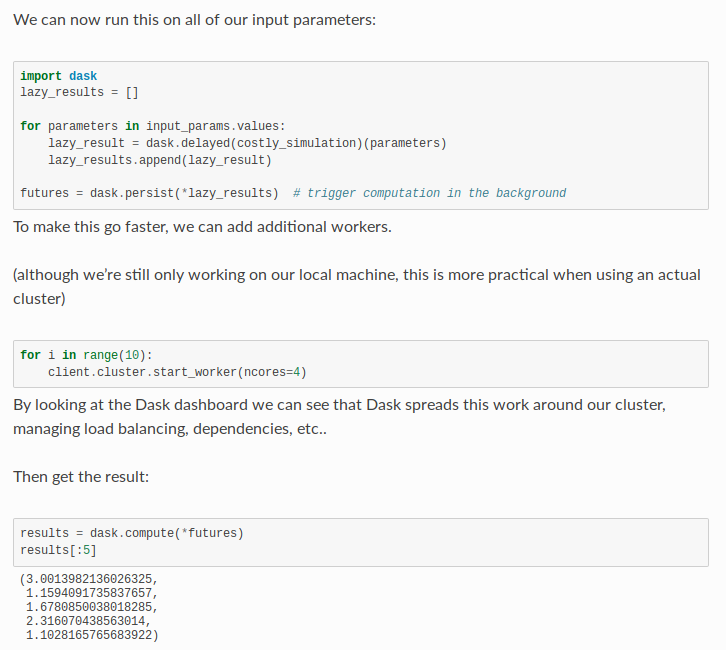
\includegraphics[width=\columnwidth]{ep_dask_code.png}
  \caption{\label{ep_dask_code} Embarrassingly parallel workload using Delayed API.}
\end{figure}

Embarrassingly parallel simulation

Before: complex and unreadable batch scripts, launching PBS arrays, writting millions of small results on shared storage.

With Dask: elegant python code, scaling easily, in memory data exchange...

Add some post processing

Add some CSV file generation, build of a dask dataframe, reduction of results, launch of a new simulation...

\subsection{Simulating remote sensing data through dask array}
\label{ssec:usecase2}

Generating a lot of Dask array that needs to be sum.
Memory problem, rechunking...


% To start a new column (but not a new page) and help balance the last-page
% column length use \vfill\pagebreak.
% -------------------------------------------------------------------------
\vfill
\pagebreak


% References should be produced using the bibtex program from suitable
% BiBTeX files 
% -------------------------------------------------------------------------

\bibliographystyle{plainnat}
\bibliography{myBibFile}

\small

\begin{thebibliography}{00}
\bibitem{b1} Abernathey, Ryan; paul, kevin; hamman, joe; rocklin, matthew; lepore, chiara; tippett, michael; et al. (2017): Pangeo NSF Earthcube Proposal. \href{https://figshare.com/articles/Pangeo_NSF_Earthcube_Proposal/5361094}{Figshare paper}. 
\bibitem{b2} Mark McInerney, ESDIS Project Deputy Project Manager/Technical: EOSDIS Cloud Evolution\href{https://earthdata.nasa.gov/about/eosdis-cloud-evolution}{NASA EOSDIS web site}. 
\bibitem{b3} Ryan Abernathey et al: \href{https://github.com/pangeo-data/pangeo/issues}{Pangeo github project issue tracker}. 
\bibitem{b4}  Joseph Hamman, Matthew Rocklin , Jim Edwards, Guillaume Eynard-Bontemps, Loïc Estève, et al. (2018): \href{https://medium.com/pangeo/dask-jobqueue-d7754e42ca53}{Scalable interactive analysis workflows using dask on HPC Systems}. 
\bibitem{b5}  Pangeo community: \href{http://pangeo.io/use_cases/index.html}{Pangeo use cases}. 
\bibitem{b6} Scott Henderson, Daniel Rothenberg, Matthew Rocklin, Ryan Abernathey, Joe Hamman, Rich Signell, and Rob Fatland: \href{https://medium.com/pangeo/cloud-native-geoprocessing-of-earth-observation-satellite-data-with-pangeo-997692d91ca2}{Cloud Native Geoprocessing of Earth Observation Satellite Data with Pangeo}. 
\bibitem{b7} Ryan Abernathey: \href{https://medium.com/pangeo/step-by-step-guide-to-building-a-big-data-portal-e262af1c2977}{Step-by-Step Guide to Building a Big Data Portal}.
\bibitem{b7} Ryan Abernathey: \href{https://medium.com/pangeo/step-by-step-guide-to-building-a-big-data-portal-e262af1c2977}{Step-by-Step Guide to Building a Big Data Portal}.
\bibitem{b8} Joe Hamman, Ryan Abernathey: \href{https://medium.com/pangeo/pangeo-meets-binder-2ea923feb34f}{Pangeo meets Binder}.
\end{thebibliography}
\end{document}
